\section{LED driver circuits}\label{sec:led-driver-circuit}

	A keen aspect of a user operated system is the capability of the system to show useful and relevant feedback data to the user \cite{laurel1990art}. This system will have a high-layer software GUI in order to show processed data to the user as it was defined in Section \ref{sec:software-requirements} in Item \ref{itm:soft-req-6}. However, some direct hardware feedback is also useful, in this project the main hardware feature to show feedback are LEDs.
	\par
	The ideia is to have LEDs that will indicate in which stage of operation the system is. It was decided to make a separate LED circuit block in order to make changes on LED's types independent from the circuit they are giving feedback. The following sections will show and explain each functionality of the system that will have LED feedback. All LEDs will be directly connect to the power supplies and just their cathodes will be connect to the drivers circuit.
		
	\subsection{Serial Communication Leds}\label{ssec:serial-communication-leds}
		One important feature of the system is it's serial communication, this is the only way the MCU will communicate with the outside world, as was explained in Section \ref{sec:hardware-interface-between-mcu-and-computer}. In Section \ref{ssec:usb-uart-complete-circuit} it was said that nets \textit{TX$\_$CON} and \textit{RX$\_$CON} from Figure \ref{fig:usb-uart-circuit} are open drain input when the system is respectively transmitting and receiving serial data and high-impedance ports when they are not communicating.
		\par
		The system will have a LED to indicate transmission and another for reception of serial data, the solution to drive this LEDs will be the NTZD3152PT1H from \textit{ON Semiconductor} \cite{ntzd3152pt1h-datasheet}. This is a dual P-Channel mosfet in one IC with very low maximum\textit{Gate Threshold Voltage} ($V_{GS}=-1V$), as the USB/UART feedback pins drains current when communicating, by connecting theese pins to the Gate of theese PMOS it will be possible to control when the LEDs will be turned on. Figure \ref{fig:leds-uart} show this circuit configuration implemented.

		\begin{figure}[htbp]
			\centering
				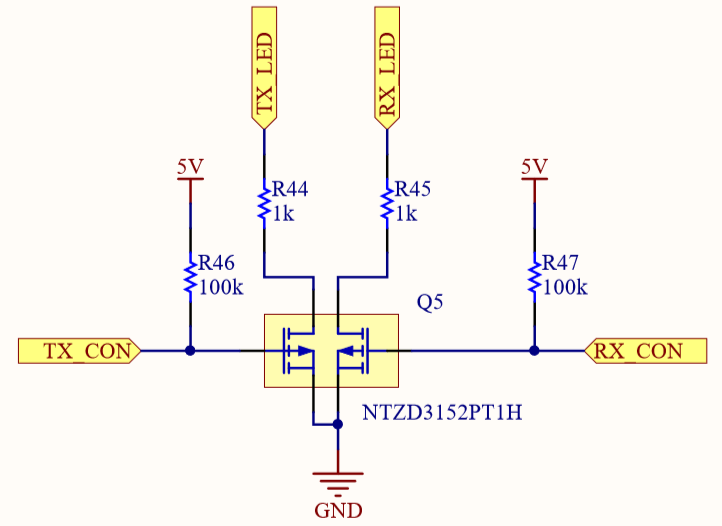
\includegraphics[scale=1.3]{figuras/fig-leds-uart.png}
			\caption{UART feedback LEDs driver \cite{leds-uart}}
			\label{fig:leds-uart}
		\end{figure}

		The resistors R44 and R45 are current limiting resistors, there value may vary with the choosen LEDs, so this 1k$\omega$ value is not necessary fixed. Resistors R46 and R47 have a relatively bigger resistance of 100k$\omega$ because they are pull-up resistos, they do not control current on that port, they were used just to guarantee that the voltage on the gate of the PMOS is higher than 1V (Gate-Source Threshold Voltae of the transistors according to the NTZD3152PT1H datasheet \cite{ntzd3152pt1h-datasheet}) when the UART/USB IC is turned off (in Section \ref{ssec:usb-uart-conversion-circuit} a possible scenario that the IC is not turned on is presented).

	\subsection{Sensor Disconnection and Acquisition Leds}\label{ssec:sensor-disconnection-acquisition-leds}	

		\subsubsection{Sensor Disconnection}\label{sssec:sensor-disconnection-leds}

			As it was defined in Item \ref{itm:func-req-14} from Section \ref{sec:functionalRequirements}, the system needs to be able to detect when a sensor is disconnected. Moreover, every sensor in this project has a net that goes to high-logic level (5V, according to Section {ssec:the-choosen-mcu}) and this signal can be used to activate LEDS to indicate wheter each sensor is connected or not.

		\subsubsection{Acquisition}\label{sssec:acquisition-led}

			The major funcition of this project is to make a acquisition system, so the major activity from the MCU is acquiring data. So, to give some feedback to the user a LED was reserved just for the MCU to indicate if the system is acquiring data or not. The control of this LED is controlled directly from the MCU, so if any extra functionality is desired to be implement, no hardware change will need to be carried out, just code.

		\subsubsection{Sensor Disconnection and Acquisition LED driver}\label{sssec:sensor-disconnection-and-acquisition-led-driver}

			As the sensor disconnection LEDs and the acquisition LED are all activated when high-logic level is present on their respective activation nets, the same solution can be applied. The choosen alternative to drive this LEDs is the TPL7407LAPWR from \textit{Texas Instruments} \cite{TPL7407LAPWR-datasheet}, it is a low-side driver than has a high-logic voltage level of 1.5V and a low-level voltage of 0.9V. The driver drains current when a high logic level is present at each channels activation port. This driver has seven channels and can drain up to 600mA per channel, making it more than ideal to drive LEDs. As this maximum drain current is quite high, if other devices such as relays and sirens can be connected instead of the LEDs without changing the hardware project, just changing the current limiting resistors. Figure \ref{fig:leds-sensor-disconnection-acquisition-circuit} shows the circuit to drive theese LEDs, resistors R30 to R36 are the current limiting resistors mentioned above and resistors R37 to R43 pull-down resistors used just to guarantee that the logic level will remain low (driver not draining current) if there is no definitive voltage input. The capacitor C10 is just a decoupling capacitor for the IC power supply recommended by the datasheet \cite{TPL7407LAPWR-datasheet}.

			\begin{figure}[htbp]
				\centering
					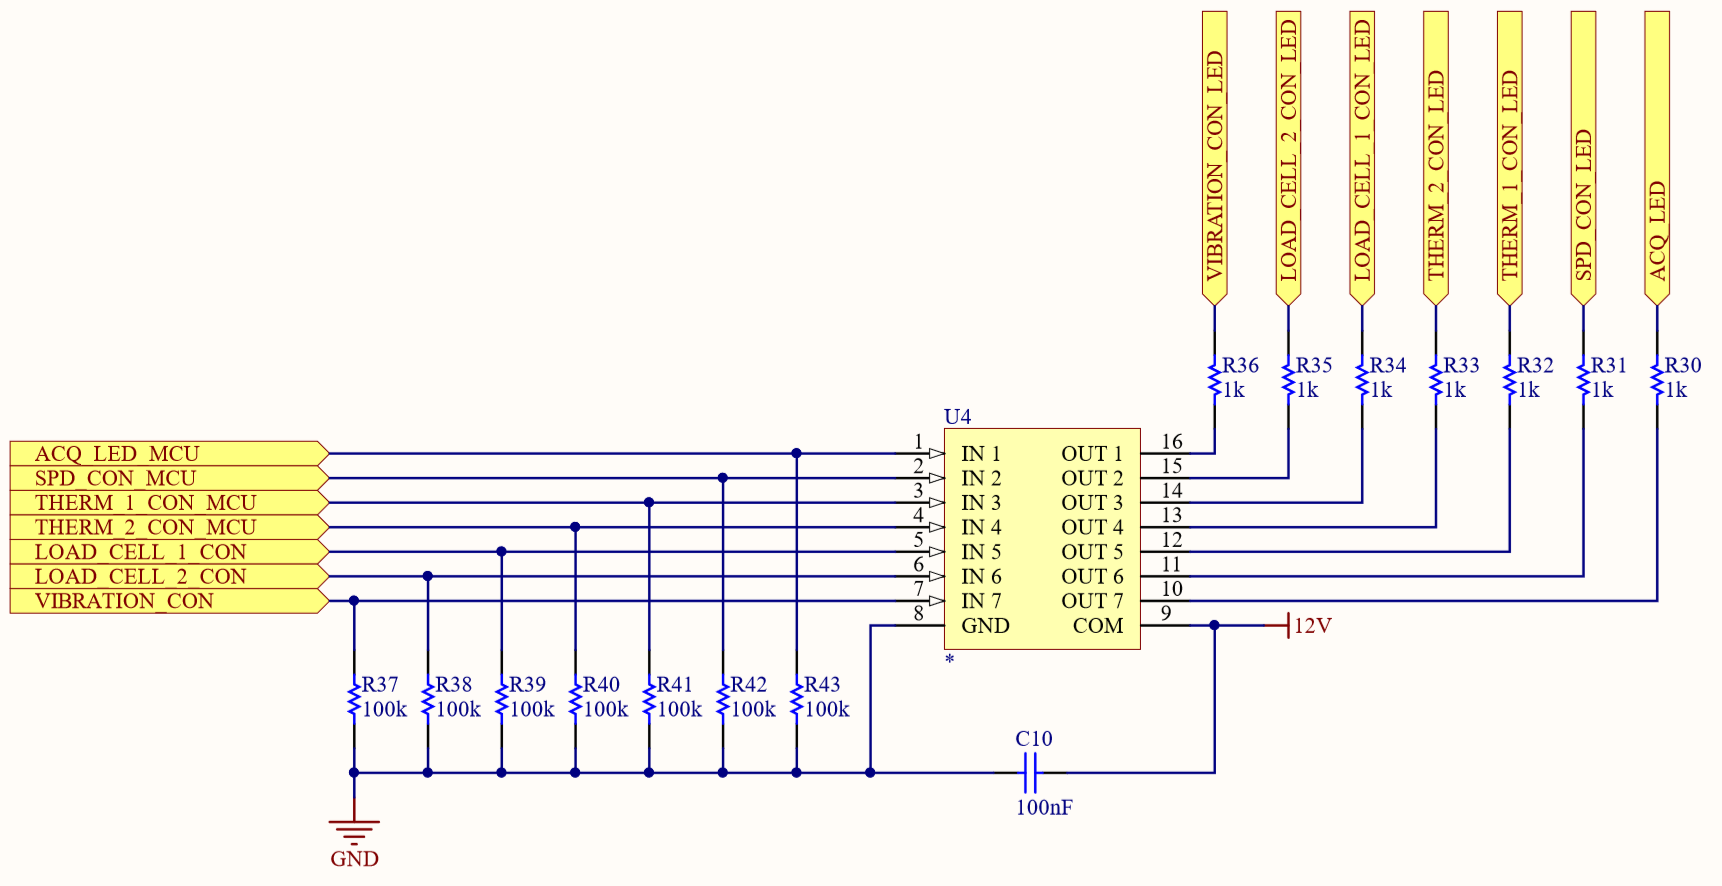
\includegraphics[scale=0.7]{figuras/fig-leds-sensor-disconnection-acquisition-circuit.png}
				\caption{Sensor Disconnection and Acquisition LED driver circuit \cite{leds-sensor-disconnection-acquisition-circuit}}
				\label{fig:leds-sensor-disconnection-acquisition-circuit}
			\end{figure}

	\subsection{Power Supplies Voltage LEDs}\label{ssec:power-supplis-voltage-leds}

		This is by far the simplest LED circuit, it is just current limiting resistors connected in series to the LEDs as Figure \ref{fig:power-supplies-leds} shows.

			\begin{figure}[htbp]
				\centering
					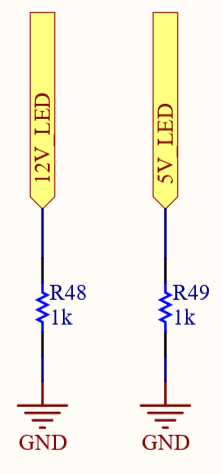
\includegraphics[scale=1.3]{figuras/fig-power-supplies-leds.png}
				\caption{Power Supplies Voltage LEDs Circuit \cite{power-supplies-leds}}
				\label{fig:power-supplies-leds}
			\end{figure}